%% SECTION HEADER /////////////////////////////////////////////////////////////////////////////////////
\section{Displacements coupling at the interface of substructures}
\label{sec:interface}

%% SECTION CONTENT ////////////////////////////////////////////////////////////////////////////////////

The present model of the sandwich panel consists of \ac{2d} and \ac{3d} elements. 
Moreover, there are non-matching grids between two adjacent substructures. 
These involve connecting them by imposing the compatibility of the displacements at the interface, see Fig.~\ref{fig:interface}.
This type of connection is implemented through the interface elements based on Lagrange multipliers, which are interpreted as forces responsible for determining the appropriate displacements of nodes \cite{fiborek20192d, fiborek2022spectral}.
The coupling can be expressed as:
\begin{eqnarray}
	\left\{\begin{array}{c}
		\textbf{u}\\
		\textbf{v}\\
		\textbf{w}
	\end{array}\right\}_{s_{i1}}^{\Gamma^i}-
	\left\{\begin{array}{c}
		\textbf{u}\\
		\textbf{v}\\
		\textbf{w}
	\end{array}\right\}_{s_{i2}}^{\Gamma^i}=
	\left\{\begin{array}{c}
		\textbf{0}\\
		\textbf{0}\\
		\textbf{0}
	\end{array}\right\},
	\label{eq:coupling}
\end{eqnarray}
\nomtypeD[Gamma]{$\Gamma$}{Interface}{}%
\begin{figure}
	\begin{center}
		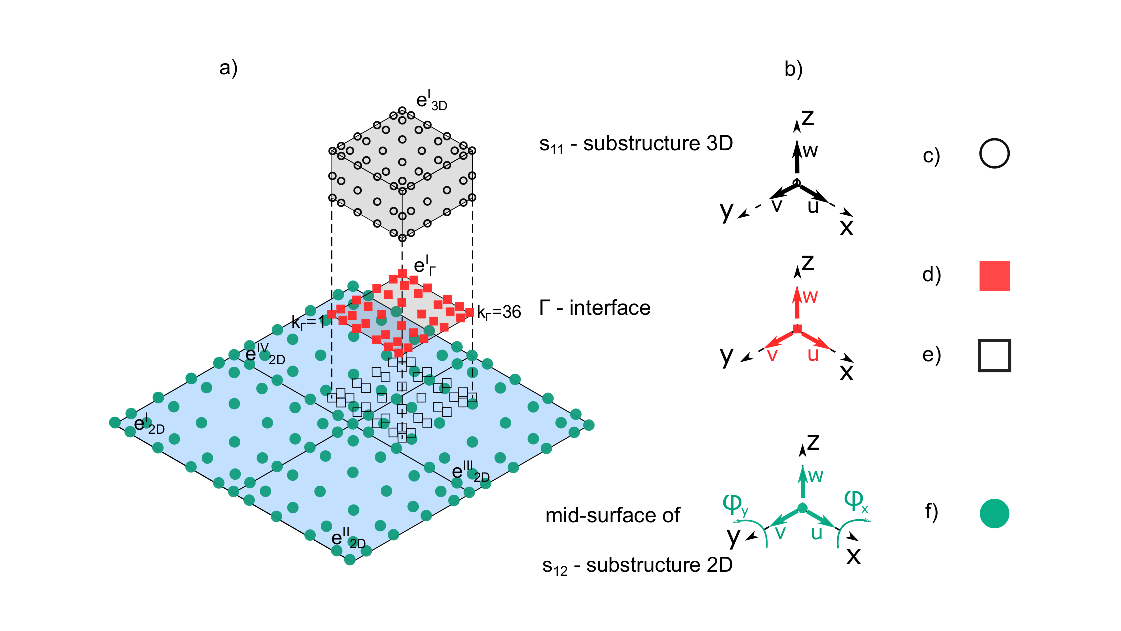
\includegraphics[width=0.95\textwidth]{Chapter_4/interface_2D3D}
	\end{center}
	\caption{Non-matching interface setup: a) interface coupling, b) degrees-of-freedom of the interface and the substructures.}
	\label{fig:interface}
\end{figure}
where \(s_{i1}\) and \(s_{i2}\) are substructures connected by the interface \(\Gamma^i\). For the whole structure, the Eq.~(\ref{eq:coupling}) can be written in the matrix form:
\begin{eqnarray}
	\textbf{G}\textbf{d}=\textbf{0},
	\label{eq:cond_disp}
\end{eqnarray}
\nomtypeD[G]{$\textbf{G}$}{Interface coupling matrix}{}%
where \textbf{G} is the coupling matrix which contains the equations to interpolate the substructures displacements at the interfaces, and \(\textbf{d}\) is a global displacement field for \(nS\) number of substructures, composed as:
\begin{eqnarray}
	\textbf{d} = \left\{\begin{array}{cccc}
		\textbf{d}_1, & \textbf{d}_2, &\ldots, & \textbf{d}_{nS}
	\end{array}\right\}^T.
	\label{eq:displacements}
\end{eqnarray}

General formulation of the matrix \textbf{G} is presented in Algorithm \ref{alg:G_matrix}.

\begin{algorithm}[H]
	\SetAlgoLined
	\For{i = 1 \KwTo 2}{
		create \(n^{\Gamma}\times n^{s_i}\) null matrix 
		\(\mathbf{G}_i\),\\
		\For{j = 1 \KwTo \(n^{\Gamma}\)} {
			find \(ownerElement^j_i\) in the structure \(s_i\) 
			containing interface node \(j\) with global coordinates vector: 
			\(X_p=(x^j_p,y^j_p)\)\;
			assign vector \(X_e=(x_e,y_e)\) of coordinates of all nodes in 
			\(ownerElement^j_i\)\;
			assign initial coordinates 
			\(X_{\kappa}=(x^j_{\kappa},y^j_{\kappa})\) to the nearest node in
			\(ownerElement^j_i\) to node \(j\)\;
			transform global coordinates \(X_{\kappa}\) to a local coordinate system \(\xi_{\kappa}=\xi(X_{\kappa});\quad 
			\eta_{\kappa}=\eta(X_{\kappa})\)\;
			\While{\(\left|X_p-X_{\kappa}\right|>\mathrm{tol}\)}{
				\(\xi_{\kappa+1}=\xi_{\kappa}+(\mathcal{J}_{\kappa})^{1,1}_{\mathrm{inv}}.*(x^j_p-x_{\kappa}^j)
				+(\mathcal{J}_{\kappa})^{1,2}_{\mathrm{inv}}.*(y^j_p-y_{\kappa}^j)\)\;
				\(\eta_{\kappa+1}=\eta_{\kappa}+(\mathcal{J}_{\kappa})^{2,1}_{\mathrm{inv}}.*(x^j_p-x_{\kappa}^j)
				+(\mathcal{J}_{\kappa})^{2,2}_{\mathrm{inv}}.*(y^j_p-y_{\kappa}^j)\)\;
				\(X_{\kappa}=N_{\kappa+1}X_e\)\;
			}
			\(\mathbf{G}_i(j,n^{X_e})=N_{\kappa+1}\)\;
		}
		\uIf{\(s_i\) \(\mathrm{is\ 3D}\)} {
			\(\mathbf{G}_i=\left[\begin{array}{ccc}
				\mathbf{G}_i & \mathbf{0} & \mathbf{0}\\
				\mathbf{0} & \mathbf{G}_i & \mathbf{0}\\
				\mathbf{0} & \mathbf{0} & \mathbf{G}_i
			\end{array} \right]
			\)\;
		}
		\ElseIf{\(s_i\) \(\mathrm{is\ 2D}\)} {
			\(\mathbf{G}_i=\left[\begin{array}{ccccc}
				\mathbf{G}_i & \mathbf{0} & \mathbf{0} & 
				\frac{h_i}{2}\mathbf{G}_i & \mathbf{0}\\
				\mathbf{0} & \mathbf{G}_i & \mathbf{0} & \mathbf{0} & 
				\frac{h_i}{2}\mathbf{G}_i\\
				\mathbf{0} & \mathbf{0} & \mathbf{G}_i & \mathbf{0} & 
				\mathbf{0}
			\end{array} \right]\)\;
		}
	}
	
	\KwResult{coupling matrix \(\mathbf{G}=\left[\begin{array}{cc}
		\mathbf{G}_1 & \mathbf{G}_2
	\end{array} \right]\)}
	\caption{Interface coupling matrix formulation}
	\label{alg:G_matrix}
\end{algorithm}
\nomtypeD[Jacobian]{$\mathcal{J}$}{Jacobian matrix}{}%
\nomtypeD[n]{$n$}{Nodes number}{-}%
\nomtypeR[Xp]{$X_p$}{Coordinates vector of the interface point}{}{\unit{\metre}}%
\nomtypeR[Xe]{$X_e$}{Coordinates vector of the element nodes}{}{\unit{\metre}}%
where \(s_i\) is one of the coupled structures, \(n^{\Gamma}\) and \(n^{s_i}\) are node numbers of the interface and node numbers of the structure \(s_i\), respectively; \(\left(\mathcal{J}_{\kappa}\right)_{\mathrm{inv}}\) is the inverse Jacobian matrix evaluated at \((\xi_{\kappa},\eta_{\kappa})\) and \(N_{\kappa+1}\) is the shape function evaluated at \((\xi_{\kappa+1},\eta_{\kappa+1})\), \(n^{X_e}\) is the vector of global order numbers of all nodes in the \(ownerElement^j_i\), \(h_i\) is a thickness of the structure \(s_i\) and \(tol\) is a termination criterion for iterations.

The main task of the algorithm is to calculate shape functions for each adjacent substructure at the points \(X_p=(x_p^k,y_p^k)\), which are projections of the interface nodes onto these substructures.
The shape function can be calculated after finding an owner element and local coordinates of the points.
Owner element is a spectral element in the domain of the substructure \(s_{ij}\) which contains interface node, for example, interface node \(k_\Gamma=36\) (see~Fig.~\ref{fig:interface}a)) is located in the element \(e^{I}_{3\mathrm{D}}\) and \(e^{III}_{2\mathrm{D}}\) for the substructures \(s_{11}\) and \(s_{12}\), respectively.
It can be found within two ways: using Matlab's built-in function \verb+inpolygon+ or more efficient procedure proposed by Silva et al. \cite{silva2009exact} which was used in the current implementation.
In this procedure, an initial approximation is first performed by rejecting all external points outside the rectangular region bounded by the points \(\mathrm{P_{min}}\) and \(\mathrm{P_{max}}\) as shown in Fig. \ref{fig:b_b_test}(\textbf{a}).
If \(\mathrm{X_p}\) is inside the element, then the vectors \(\vec{V}_1\) and \(\vec{V}_2\) have the same direction.
\(\vec{V}_1\) and \(\vec{V}_2\) are defined as:
\begin{eqnarray}
	\vec{V}_1 & = & \vec{v}_1\times \vec{v}_p,\\
	\vec{V}_2 & = & \vec{v}_p\times \vec{v}_2.
\label{eq:v_vectors}
\end{eqnarray}
\nomtypeD[vvv]{$\vec{v}_p,\,\vec{v}_1,\,\vec{v}_2$}{Cross-product test  vectors}{}%
\nomtypeD[V1]{$\vec{V_1}$}{First cross-product vector}{}%
\nomtypeD[V2]{$\vec{V_2}$}{Second cross-product vector}{}%

The vectors \(\vec{v}_p\), \(\vec{v_1}\) and \(\vec{v_2}\) are pictured in Fig. \ref{fig:b_b_test}(\textbf{b}). \(\vec{V}_1\) and \(\vec{V}_2\) will have the same direction if the inequality is satisfied for each element vertex \(i\):
\begin{eqnarray}
		\vec{V}_1 \cdot \vec{V}_2 \geq0,
	\label{eq:dot_prod}
\end{eqnarray}
then, the transformation from global to local coordinates is realised by the iterative method presented in the work of Li et al.~\cite{li2014efficient} (see also \verb+while-loop+ in Alg. \ref{alg:G_matrix}).
\begin{figure}[H]
	\begin{center}
		\includegraphics[width=0.95\textwidth]{Chapter_4/b_b_test}
	\end{center}
	\caption{Owner element for Xp interface node (\textbf{a}) boundary test, (\textbf{b}) cross-product test}
	\label{fig:b_b_test}
\end{figure}
While the cross-product test is exact for elements with linear edges, the approximation of the boundary test is used for second order elements, and then \(\xi_{\kappa}\) and \(\eta_{\kappa}\) must satisfy the condition \(-1\leq \xi_{\kappa},\eta_{\kappa} \leq 1\).
The computational effectiveness of Alg.~\ref{alg:G_matrix} can be easily improved if certain precautions are taken.
Firstly, the mesh of the interface has to be based on the mesh from one of the substructures \(s_{i}\), which may be referred to as a slave.
So, shape functions evaluated at (\(\xi\), \(\eta\)) may take only zero and one values.
Moreover, the code was vectorised rather than using a for-loop form, provided that the required matrix of size \(4n^e\times n^{\Gamma}\), where \(n^e\) is the number of elements of the structure \(s_i\) elements, does not exceed the operating memory.